
% 
% \documentclass[article,tikz,border=3mm]{standalone}
\documentclass{article}
\usepackage{blindtext}

% setting up the margin of the paper 
\usepackage[a4paper, total={6.5in, 9in}]{geometry}

% setup for font family for the title/section name, for text font you have set ti seperately
\usepackage[T1]{fontenc}
\usepackage{lmodern}

% package for tables, this package I don't why always stay at the top of the document
\usepackage{tikz}
% I don't know what is this for right now
\usepackage{mathtools,eqparbox}

% not sure for right now 
\usepackage{array}
\usepackage{blkarray, bigstrut} % matrix label

% index package 
\usepackage{imakeidx}
\makeindex % this line is mandatory

% package for basic symbol characters $/rhd$
% https://artofproblemsolving.com/wiki/index.php/LaTeX:Symbols
\usepackage{latexsym}

% system of equation (such as large bracket)
\usepackage{amsmath}
\usepackage[makeroom]{cancel} % cancel out single item by using \cancel{}
\usepackage{soul} % straight cross line not in matrix
\usepackage{nicematrix} % draw straight cross line inside matrix
\NiceMatrixOptions{
code-for-first-row = \color{red} ,
code-for-last-row = \color{red} ,
code-for-first-col = \color{blue} ,
code-for-last-col = \color{red}
} % nice matrix labeling
\usepackage{mathtools} % display fraction-like 
\newcommand\aug{\fboxsep=-\fboxrule\!\!\!\fbox{\strut}\!\!\!} % this line is for the veritical line in augmented matrix, but you can use array to achieve this as well

\usepackage{pgfplots} % 2 dimensional ploting
\pgfplotsset{compat=1.10}
\usetikzlibrary{datavisualization.formats.functions} % 2 dimensional ploting
\usetikzlibrary{tikzmark} % arrow for pointing
\usepackage{tikz-3dplot} % 3 dimensional plot
\newcommand{\Arrow}[1]{%
\parbox{#1}{\tikz{\draw[->](0,0)--(#1,0);}}
} % for \Arrow in tikz package

\hbadness=10000  % silence the warning for \\ breaking on empty line

\usetikzlibrary{automata,arrows,positioning,calc} % markov chain


% ================================================== Main.tex ==============================================
\begin{document}


% ploting the table using tikz package
\begin{table}
\[\begin{array}{c|ccccc}
\tikz{\node[below left, inner sep=1pt] (food) {Food};%
      \node[above right,inner sep=1pt] (ingredient) {Ingredient};%
      \draw (food.north west|-ingredient.north west) -- (food.south east-|ingredient.south east);}
 & Ca^{2+} & Na^{+} & Sugar & Calories \\
\hline
    rice & x_{11} & x_{12} & x_{13} & y_{1} \\
    meat & x_{21} & x_{22} & x_{23} & y_{2} \\
    fish & x_{31} & x_{32} & x_{33} & y_{3} \\
    apple & x_{41} & x_{42} & x_{43} & y_{4} \\
\end{array}\]
\caption{Nutrition Values}
\end{table}

% section start
\section{Representation of Matrix}
Table could be viewed as a matrix, below are an illustration coressponding to the above table. The 4x3 matrix stands for attributes while weights are used for calculating y (outcome)
\begin{center}
    $\begin{bmatrix}
        x_{11} & x_{12} & x_{13} \\
        x_{21} & x_{22} & x_{23} \\
        x_{31} & x_{32} & x_{33} \\
        x_{41} & x_{42} & x_{43} \\
    \end{bmatrix}$
    x 
    $\begin{bmatrix} 
        w_{1} \\ 
        w_{2} \\
        w_{3} \\
    \end{bmatrix}$
    =
    $\begin{bmatrix} 
        y_{1} \\ 
        y_{2} \\
        y_{3} \\
        y_{4} \\
    \end{bmatrix}$ \\
\end{center}

% only centering centain text
\centerline{matrix multiplication(dim): 4x3 • 3x1 = 4x1}

% subsection
\subsection{In general}
\text{Like numbers, matrices can be added, subtracted, multiplied, and divided} \\
\text{matrices have many other uses in mathematics and the sciences, knowing matrix algebra is essential}

% new section 
\section{Matrix Properties}
\subsection{Equality}
The matrices A = $[a_{ij}]$ and B = $[b_{ij}]$ are equal if and only if \\ 
• they have the same dimension m x n \\ 
• corresponding entries are equal $a_{ij} = b_{ij}$: for i=1, 2, ... ,m and j=1, 2, ... ,n 


% stretch the size of the table in vertical level
\begin{center}
    \renewcommand{\arraystretch}{4}

    \begin{tabular}{|*2{>{\renewcommand{\arraystretch}{1}}c|}}
    \hline
    \textbf{Equal} & \textbf{Unequal}\\
    \hline
    $ \left[ \begin{array}{ccc} \sqrt{4} & 2^2 & e^0 \\ 0.5 & 1 & 1-1 \end{array}\right]$ = $ \left[ \begin{array}{ccc} 2 & 4 & 1 \\ \frac{1}{2} & \frac{2}{2} & 0 \end{array}\right]$  & 
    $ \left[ \begin{array}{cc} 1 & 2 \\ 3 & 4 \\ 5 & 6 \end{array}\right]$ $\neq \left[ \begin{array}{ccc} 1 & 3 & 5 \\ 2 & 4 & 6 \end{array}\right]$ \\
    \hline
    \end{tabular} 
\end{center}

• Find a, b, c, and d if 
$\begin{bmatrix}
    a & b \\ 
    c & d
\end{bmatrix}$
= 
$\begin{bmatrix}
    1 & 3 \\ 
    5 & 2
\end{bmatrix}$. 
In order for two matrices to be equal, we have a=1, b=3, c=5, d=2


\subsection{Addition, Subtraction, and Scalar Multiplication}

Let A = $[a_{ij}]$ and B = $[b_{ij}]$ be matrices of the \textbf{same dimension} m x n, c be any real number \\
\indent 1) addition: A + B = $[a_{ij} + b_{ij}]$ \\
\indent 2) subtraction: A - B = $[a_{ij} - b_{ij}]$ \\ 
\indent 3) scalar product: cA = $[ca_{ij}]$

\subsection{Multiplcation of Matrices}
The product AB (or A•B) of two matrices A and B is defined only when the number of columns in A is equal to the number of rows in B 



\begin{center}
  \begin{tabular}{ | l | c | r |}
    \hline
    Matrices & A & B \\ \hline
    Dimensions & m x \textbf{n} & \textbf{n} x k \\ 
    \hline
  \end{tabular} \\
\end{center}
\centerline{n is the columns in A, rows in B, the new resulting matrix has the dimension of \textbf{m x k}} 

\begin{itemize}
    \item[$>>$] \textbf{Inner Product} \\
    if $[a_1 a_2 \hdots a_n]$ is a row of A, and if 
    $\begin{bmatrix} 
        b_1 \\ 
        b_2 \\ 
        \vdots \\
        b_n \\
    \end{bmatrix}$
    is a column of B, their inner product is the number \\ $\mathbf{a_1b_1 + a_2b_2 + \hdots + a_nb_n}$

    \item[$>>$] \textbf{ex)} \\ 
    $\begin{bmatrix} 
        2 & -1 & 0 & 4
    \end{bmatrix}$
    and 
    $\begin{bmatrix} 
        5 \\ 
        4 \\ 
        -3 \\
        \frac{1}{2} \\
    \end{bmatrix}$
    gives: 2•5 + (-1)•4 + 0•(-3) + 4• $\frac{1}{2}$ = 8

    \item[$>>$] $\mathbf{c_{ij}}$ \\ 
    based on the examples, the resulting formula for matrices multiplcation with multi-entry

    $\begin{bmatrix} 
        a_{11} & a_{12} \\ 
        a_{21} & a_{22} \\ 
    \end{bmatrix}$
    • 
    $\begin{bmatrix} 
        b_{11} & b_{12} & b_{13} \\ 
        b_{21} & b_{22} & b_{23} \\ 
    \end{bmatrix}$
    = \\
    $\begin{bmatrix} 
        c_{11}(a_{11}*b_{11} + a_{12}*b_{21}) & c_{12}(a_{11}*b_{12} + a_{12}*b_{22}) & c_{13}(a_{11}*b_{13} + a_{12}*b_{23}) \\ 
        c_{21}(a_{21}*b_{11} + a_{22}*b_{21}) & c_{22}(a_{21}*b_{12} + a_{22}*b_{22}) & c_{23}(a_{21}*b_{13} + a_{12}*b_{23}) \\ 
    \end{bmatrix}$

\end{itemize}


\subsection{Properties of Matrix Multiplication}

$\rhd$ Order Matters \\
\indent 1) $A^2 - B^2 = (A+B)(A-B)$ {\color{red}False: expand and do the calculation}  \\
\indent 2) $(A+B)^2 = A^2 + 2AB + B^2$ {\color{red}False: found order changed after expanding} \\
\indent 3) $(A-B)^2 = A^2 - 2AB + B^2$ {\color{red}False: found order changed after expanding}  \\
\indent 4) $(AB)^2 = A^2B^2$ {\color{red}False: (AB)(AB) = ABAB, there is BA discomfort with original order} \\
\indent 5) $(kA)(kB) = k^2(AB)$ {\color{green}True}


\subsection{Application of Matrix Multiplcation}

$\begin{bmatrix} 
    1 & -1 & 3 \\ 
    1 & 2 & -2 \\ 
    3 & -2 & 5 \\ 
\end{bmatrix}$
• 
$\begin{bmatrix} 
    x \\
    y \\ 
    z \\
\end{bmatrix}$
= 
$\begin{bmatrix} 
    4 \\
    10 \\ 
    14 \\
\end{bmatrix}$
becomes this
$\begin{bmatrix} 
    x & -y & 3z \\ 
    x & 2y & -2z \\ 
    3x & -y & 5z \\ 
\end{bmatrix}$
=
$\begin{bmatrix} 
    4 \\
    10 \\ 
    14 \\
\end{bmatrix}$
\\
\textbf{it becomes the system of linear equation}
$\begin{cases}
    x-y+3z = 4 \\ 
    x+2y-2z = 10 \\ 
    3x-y+5z = 14 \\ 
\end{cases}$

% ------------ different way of writing system of equation -------------
% \begin{equation*}
%   \left\{
%     \begin{aligned}
%       & x-y+3z = 4 \\
%       & x+2y-2z = 10 \\
%       & 3x-y+5z = 14 \\
%       % & {\left|
%       %   \frac{k_{p\omega}s + k_{i\omega}}{s} \cdot \frac{1}{Ts + 1}
%       % \right|}_{s = j \cdot 2\pi} = 1
%     \end{aligned}
%   \right.
% \end{equation*}
% ----------------------------------------------------------------------


\subsection{Matrix Transpose}

1) A: $\begin{bmatrix} x_1 & x_2 & x_3 \end{bmatrix}$ is a 1x3 matrix $\rightarrow$ $A^T$: $\begin{bmatrix} x_1 \\ x_2 \\ x_3 \end{bmatrix}$ becomes a 3x1 matrix \\
2) A square Matrix A is symmetric if x = $x^T$, visual representation: $\begin{bmatrix} a & b \\ c & d \end{bmatrix} \rightarrow$ $\begin{bmatrix} a & c\\ b & d \end{bmatrix}$\\
3) A = $\begin{bmatrix} 1 & 5 \\ 5 & 1 \end{bmatrix}$ = $A^T$ = $\begin{bmatrix} 1 & 5 \\ 5 & 1 \end{bmatrix}$ \\
4) matrix operation with transpose: $\begin{cases} (A^T)^T = A \\ (A+B)^T = A^T + B^T \\ (AB)^T = B^TA^T \\ (cA)^T = c(A^T) \end{cases}$




\section{Determinants}

If a matrix is square (rows = columns), then we can assign to it a number called its determinant. \\ 
\indent >> determinant can be used to solve systems of linear equation \\
\indent >> useful in determining whether a matrix has an inversse \\ 
\indent >> denote by det(A) or |A|

\subsection{Determinants of 2 x 2 Matrix}
A = $\begin{bmatrix} a & b \\ c & d \end{bmatrix}$ is: det(A)= $\begin{vmatrix} a & b \\ c & d \end{vmatrix}$ = ad - bc \\ 
B = $\begin{vmatrix} 6 & -3 \\ 2 & 3 \end{vmatrix}$, det(B) = 6•3-(-3)•2 = 18 -(-6) = 24


\subsection{Determinants of n x n Matrix}
If A is an n x n matrix, the determinant of A is obtained by multiplying each element of the first row by its cofactor, and then adding the result, below is the general form 
\begin{itemize}

    \item[>>] cofactor: the determinant for chosen element with row and column are crossed out(denoted by $a_{ij}$)
    \item[>>] GF => expand the first row: det(A)=|A|= $\begin{vmatrix}
                                        a_{11} & a_{12} & \hdots & a_{1n} \\ 
                                        a_{21} & a_{22} & \hdots & a_{2n} \\
                                        \vdots & \vdots & \ddots & \vdots \\
                                        a_{n1} & a_{n2} & \hdots & a_{nn}
                                    \end{vmatrix} = a_{11}A_{11} + a_{12}A_{12} + \hdots + a_{1n}A_{1n}$ 
    \item[>>] use 3x3 matrix as example: A = $\begin{vmatrix} 2 & 3 & -1 \\ 0 & 2 & 4 \\ -2 & 5 & 6 \end{vmatrix}$ while the positive and negative sign of $a_{ij}$ 
              is determined by checking the odd or even of (i+j), like this $\begin{bmatrix} + & - & +  \\ - & + & - \\ + & - & + \end{bmatrix}$
    \item[>>] expand the first row
    \begin{itemize}
        \item[1)] $A_{11}$ = 2
            $\begin{pNiceMatrix} 
                  2 & 3 & -1 \\ 
                  0 & 2 & 4 \\ 
                  -2 & 5 & 6 
                  \CodeAfter 
                  \begin{tikzpicture}
                     \draw [thick,red] (1-1.west) -- (1-3.east); 
                     \draw [thick,red] (1-1.north) -- (3-1.south); 
                  \end{tikzpicture}
              \end{pNiceMatrix}$
              = 2 $\begin{vmatrix} 2 & 4 \\ 5 & 6 \end{vmatrix}$

        \item[2)] $A_{12}$ = -3  
              $\begin{pNiceMatrix}
                  2 & 3 & -1 \\ 
                  0 & 2 & 4 \\ 
                  -2 & 5 & 6 
                  \CodeAfter 
                  \begin{tikzpicture}
                     \draw [thick,red] (1-1.west) -- (1-3.east); 
                     \draw [thick,red] (1-2.north) -- (3-2.south); 
                  \end{tikzpicture}
              \end{pNiceMatrix}$
              = -3 $\begin{vmatrix} 0 & 4 \\ -2 & 6 \end{vmatrix}$

        \item[3)] $A_{12}$ = -3  
              $\begin{pNiceMatrix}
                  2 & 3 & -1 \\ 
                  0 & 2 & 4 \\ 
                  -2 & 5 & 6 
                  \CodeAfter 
                  \begin{tikzpicture}
                     \draw [thick,red] (1-1.west) -- (1-3.east); 
                     \draw [thick,red] (1-3.north) -- (3-3.south); 
                  \end{tikzpicture}
              \end{pNiceMatrix}$
              = -1 $\begin{vmatrix} 0 & 2 \\ -2 & 5 \end{vmatrix}$
    \end{itemize}

    det(A) = 2(2•6 - 4•5) -3[0•6-4(-2)] -[0•5-2(-2)] \\ 
    = -16-24-4 \\
    = -44

    \item[>>] you can expand a whole row or column in either direction, not only the first row, you can also use the last column something like that -> Same result.
\end{itemize}

\subsection{Invertibility}
if A is a square matrix, then A has an inverse if and only if det(A) $\neq$ 0 \\
\indent >> ex. show that the matrix A has no inverse A=$\begin{bmatrix} 1 & 2 & 0 & 4  \\ 0 & 0 & 0 & 3 \\ 5 & 6 & 2 & 6 \\ 2 & 4 & 0 & 9\end{bmatrix} = 
-0 \times A_{21} + 0 \times A_{22} - 0 \times A_{23} + 3 \times A_{24} = 3A_{24} = 3 \begin{vmatrix} 1 & 2 & 0 \\ 5 & 6 & 2 \\ 2 & 4 & 0 \end{vmatrix} = 3(-2) \begin{vmatrix} 1 & 2 \\ 2 & 4 \end{vmatrix}
3(-2)(1 \times 4-2 \times 2) = 0$

\indent >> since the determinant = zero, so the matrix doesn't have an inverse 

\indent >> usually we span the first row for calculating determinants of matrix that is greater than 2 dimensions with nested operation, 
but you can do that will any rows or columns as long as it is the consistent row/column for nested operations, choose rows/columns with more zeros, which will make the calculation easier


\section{Cramer's Rule}

\indent The solutions of linear equations can sometimes be expressed using determinants, refer to the following example 

\indent >> $\begin{cases} ax + by = r \\ cx + dy = s \end{cases}$ solve the this for the variable x.

\indent >> To elimninate the varible y, we multiply the first equation by d and the second by b, and subtract: 
\begin{align*} adx + bdy = rd \\ bcx + bdy = bs \\ \mathclap{\rule{6cm}{0.3pt}}\\ adx-bcx = rd-bs \end{align*}

\indent >> assume that ad-bc $\neq$ 0, we can now solve this equation for x: $x = \frac{rd-bs}{ad-bc}$, and for y: $y = \frac{as-cr}{ad-bc}$
\indent >> since the numerator and denominator of the fractions for x and y are determinants of 2 x 2 matrices, so we can express in the following way: \\
$\begin{cases}  ax + by = r \\ cx + dy = s \end{cases}$ has the solution $x = \frac{\begin{vmatrix} r & b \\ s & d \end{vmatrix}}{\begin{vmatrix} a & b \\ c & d \end{vmatrix}}, 
y = \frac{\begin{vmatrix} a & r \\ c & s \end{vmatrix}}{\begin{vmatrix} a & b \\ c & d \end{vmatrix}},$ provided $\begin{vmatrix} a & b \\ c & d \end{vmatrix} \neq 0$

\indent >> Cramer's Rule: $D = \begin{bmatrix} a & b \\ c & d \end{bmatrix}$, $D_x = \begin{bmatrix} r & b \\ s & d \end{bmatrix}$, $D_y = \begin{bmatrix} a & r \\ c & s \end{bmatrix}$. 
The solution can be written as: $x = \frac{|D_x|}{|D|}$ and $y = \frac{|D_y|}{|D|}$

\indent >> ex. solve the following system using Cramer's Rule: $\begin{cases} 2x + 6y = -1(r) \\ x + 8y = 2(s) \end{cases}$

\begin{center}
    $|D| = \begin{vmatrix} 2 & 6 \\ 1 & 8 \end{vmatrix} = 2 \cdot 8 - 6 \cdot 1 = 10$  \\ 
    $|D_x| = \begin{vmatrix} -1 & 6 \\ 2 & 8 \end{vmatrix} = (-1) \cdot 8 - 6 \cdot 2 = -20$ \\ 
    $|D_y| = \begin{vmatrix} 2 & -1 \\ 1 & 2 \end{vmatrix} = 2 \cdot 2 - (-1) \cdot 1 = 5$
\end{center}

\indent >> the solution is $x = \frac{|D_x|}{|D|} = \frac{-20}{20} = -2$ and $y = \frac{|D_y|}{|D|} = \frac{5}{10} = \frac{1}{2}$


\section{Inverse of the Matrix}
A square matrix M is invertible or non-singlar if there exist a matrix B such that A•B = I

\subsection{Identity Matrix}
In linear algebra, the \textbf{identity matrix} of size n is the n x n \textbf{square matrix} with \textbf{ones} on the \textbf{main diagonal} and \textbf{zeros} elsewhere, denoted by $I_n$ \\
\indent >> $I_1$=[1], $I_2=\begin{bmatrix} 1 & 0 \\ 0 & 1 \end{bmatrix}$, $I_3=\begin{bmatrix} 1 & 0 & 0 \\ 0 & 1 & 0 \\ 0 & 0 & 1 \end{bmatrix}$, $\hdots$ ,
$I_n=\begin{bmatrix} 1 & 0 & 0 & \hdots & 0 \\ 0 & 1 & 0 & \hdots & 0 \\ 0 & 0 & 1 & \hdots & 0 \\ \vdots & \vdots & \vdots & \ddots & \vdots \\ 0 & 0 & 0 & \hdots & 1 \end{bmatrix}$


\indent >> A = $\begin{bmatrix} 2 & 1 \\ 5 & 3 \end{bmatrix}$, B = $\begin{bmatrix} 3 & -1 \\ -5 & 2 \end{bmatrix}$, verify the inverse of a matrix (both AB = I and BA = I)\\ 
\indent A $\cdot$ B = $\begin{bmatrix} 2 & 1 \\ 5 & 3 \end{bmatrix} \cdot \begin{bmatrix} 3 & -1 \\ -5 & 2 \end{bmatrix} = 
\begin{bmatrix} 2 \cdot 3 + 1(-5) & 2(-1) + 1 \cdot 2 \\ 5 \cdot 3 + 3(-5) & 5(-1) + 3 \cdot 2 \end{bmatrix} = \begin{bmatrix} 1 & 0 \\ 0 & 1 \end{bmatrix}$


\subsection{Inverse of 2 x 2 Matrix}

If A = $\begin{bmatrix} a & b \\ c & d \end{bmatrix}$, then $A^{-1} = \frac{1}{ad - bc} \begin{bmatrix} d & -b \\ -c & a \end{bmatrix}$, remember to verify that $AA^{-1} = A^{-1}A = I$

\subsection{Inverse of n x n Matrix}

Let A be the matrix A $\begin{bmatrix} 1 & -2 & -4 \\ 2 & -3 & -6 \\ -3 & 6 & 15 \end{bmatrix}$. (a) Find $A^{-1}$. (b) Verify that $AA^{-1} = A^{-1}A = I$.

\indent a).
\begin{align*} 
\left(
\begin{array}{rrr|rrr} 
    1 & -2 & -4 & 1 & 0 & 0 \\ 
    2 & -3 & -6 & 0 & 1 & 0 \\
    -3 & 6 & 15 & 0 & 0 & 1 \\ 
\end{array}
\right)
&\xrightarrow[R_3+3R_1 \to R_3]{R_2-2R_1 \to R_2} 
\left(
\begin{array}{rrr|rrr} 
    1 & -2 & -4 & 1 & 0 & 0 \\ 
    0 & 1 & 2 & -2 & 1 & 0 \\
    0 & 0 & 3 & 3 & 0 & 1 \\ 
\end{array}
\right) \\[5pt]
&\xrightarrow{\frac{1}{3}R_3 \to R_3} 
\left(
\begin{array}{rrr|rrr} 
    1 & -2 & -4 & 1 & 0 & 0 \\ 
    0 & 1 & 2 & -2 & 1 & 0 \\
    0 & 0 & 1 & 1 & 0 & \frac{1}{3} \\ 
\end{array}
\right) \\[5pt]
&\xrightarrow{R_1+2R_2 \to R_1}
\left(
\begin{array}{rrr|rrr} 
    1 & 0 & 0 & -3 & 2 & 0 \\ 
    0 & 1 & 2 & -2 & 1 & 0 \\
    0 & 0 & 1 & 1 & 0 & \frac{1}{3} \\ 
\end{array}
\right) \\[5pt]
&\xrightarrow{R_2-2R_3 \to R_2}
\left(
\begin{array}{rrr|rrr} 
    1 & 0 & 0 & -3 & 2 & 0 \\ 
    0 & 1 & 0 & -4 & 1 & -\frac{2}{3} \\[2pt]
    0 & 0 & 1 & 1 & 0 & \frac{1}{3} \\ 
\end{array}
\right)
\end{align*}

\indent b). solve yourself

\section{Gaussian Elimination}
In general, to solve a system of linear equations using its \textbf{augmented matrix}, we use \textbf{elementary row operations} to arrive at a matrix in a certain form. \\
1) row-echelon form \\ 
2) reduced row-echelon 

\subsection{\underline{Row-Echelon} and \underline{Reduced Row-Echelon Form}}
A matrix is in row-echelon form if it satisfies the following conditions:
\begin{itemize}
    \item[1)] The first nonzero number in each row (reading from left to right) is 1. This is called the leading entry 
    \item[2)] The leading entry in each row is to the right of the leading entry in the row immediately above it
    \item[3)] All rows consisting entirely of zeros are at the bottom of the matrix
\end{itemize}
A matrix is in reduced row-echelon form if it is in row-echelon form, and also satisfies the following condition. 
\begin{itemize}
    \item[4)] Eveny number above and below each leading entry is a 0
\end{itemize}


\newcommand{\sunderb}[2]{
  \mathclap{\underbrace{\makebox[#1]{$\cdots$}}_{#2}}
}


\subsection{Not in Row-Echelon Form}

\begin{center}
$\begin{bNiceArray}{cccc|c}[right-margin=.4em]
    0 & \color{red}1 & -\frac{1}{2} & 0 & 7 \\ 
    \color{red}1 & 0 & 3 & 4 & -5 \\
    0 & 0 & 0 &\color{red}1 & 0.4 \\
    0 & \color{red}1 & 1 & 0 & 0 \\ 
    \CodeAfter 
    \UnderBrace[shorten,yshift=3pt]{4-1}{4-4}{\text{Leading 1's do not shift to the right in successive rows}}
\end{bNiceArray}$
\end{center}


\subsection{Correct Form}
\begin{center}
    \renewcommand{\arraystretch}{4}

    \begin{tabular}{|*2{>{\renewcommand{\arraystretch}{1}}c|}}
    \hline
    \textbf{Row-Echelon Form} & \textbf{Reduced Row-Echelon Form}\\
    \hline
    $ \left[ \begin{array}{ccccc} 
        \color{red}1 & 3 & -6 & 10 & 0 \\ 
        0 & 0 & \color{red}1 & 4 & -3 \\ 
        0 & 0 & 0 & \color{red}1 & \frac{1}{2} \\
        0 & 0 & 0 & 0 & 0
    \end{array}\right]$ & 
    $ \left[ \begin{array}{ccccc}
        \color{red}1 & 3 & 0 & 0 & 0 \\
        0 & 0 & \color{red}1 & 0 & -3 \\
        0 & 0 & 0 & \color{red}1 & \frac{1}{2} \\ 
        0 & 0 & 0 & 0 & 0 
    \end{array}\right]$  \\
    \hline
    \text{leading 1's shift to the right in successive rows} & \text{leading 1's have 0's above and below in that column} \\
    \hline
    \end{tabular} 
\end{center}


\subsection{Gaussian Elimination}
Once an augmented matrix is in row-echelon form, we can solve the corresponding linear system using back-substitution (this technique is called Gaussian Elimination) \\
step 1) Augmented Matrix \\
step 2) Row-Echelon Form \\
step 3) Back-Substitution \\
\indent >> \textbf{complete example:}
$\begin{cases}
    4x + 8y - 4z = 4 \\
    3x + 8y + 5z = -11 \\ 
    -2x + y + 12z = -17
\end{cases}$
first write the augmented matrix of the system, then use elementary row operations to put it in row-echelon form 
\begin{align*} 
\left(
\begin{array}{rrr|r} 
    4 & 8 & -4 & 4 \\ 
    3 & 8 & 5 & -11 \\
    -2 & 1 & 12 & -17 \\ 
\end{array}
\right)
&\xrightarrow{\frac{1}{4}R_1 \to R_1} 
\left(
\begin{array}{rrr|r} 
    \color{red}1 & 2 & -1 & 1 \\ 
    3 & 8 & 5 & -11 \\
    -2 & 1 & 12 & -17 \\ 
\end{array}
\right)
&\xrightarrow[R_3+2R_1 \to R_3]{R_2-3R_1 \to R_2}
\left(
\begin{array}{rrr|r} 
    \color{red}1 & 2 & -1 & 1 \\ 
    \color{red}0 & 2 & 8 & -14 \\
    \color{red}0 & 5 & 10 & -15 \\ 
\end{array}
\right) \\[5pt]
&\xrightarrow{\frac{1}{2}R_2 \to R_2}
\left(
\begin{array}{rrr|r} 
    \color{red}1 & 2 & -1 & 1 \\ 
    \color{red}0 & \color{red}1 & 4 & -7 \\
    \color{red}0 & 5 & 10 & -15 \\ 
\end{array}
\right)
&\xrightarrow{-\frac{1}{10}R_3 \to R_3}
\left(
\begin{array}{rrr|r} 
    \color{red}1 & 2 & -1 & 1 \\ 
    \color{red}0 & \color{red}1 & 4 & -7 \\
    \color{red}0 & \color{red}0 & \color{red}1 & -2 \\ 
\end{array}
\right) \\[5pt]
\end{align*}

\indent >> \textbf{Gauss-Jordan Elimination => Reduced Row-Echelon Form}
\begin{align*}
\left(
\begin{array}{rrr|r} 
    1 & 2 & -1 & 1 \\ 
    0 & 1 & 4 & -7 \\
    0 & 5 & 10 & -15 \\ 
\end{array}
\right)
&\xrightarrow[R_1+R_3 \to R_1]{R_2-4R_3 \to R_2}
\left(
\begin{array}{rrr|r} 
    1 & 2 & \color{red}0 & -1 \\ 
    0 & 1 & \color{red}0 & 1 \\
    0 & 0 & 1 & -2 \\ 
\end{array}
\right)
&\xrightarrow{R_1-2R_2 \to R_1}
\left(
\begin{array}{rrr|r} 
    1 & \color{red}0 & \color{red}0 & -3 \\ 
    0 & 1 & \color{red}0 & 1 \\
    0 & 0 & 1 & -2 \\ 
\end{array}
\right)\\[5pt]
\end{align*}
The solution set becomes: $\begin{cases} x = -3 \\ y = 1 \\ z = -2 \end{cases}$

\section{Inconsistent and Dependent System}
Suppose the augmented matrix of a system of linear equations has been transformed by Gaussian elimination into row-echelon form. Then, exactly one of the following is true:
\begin{itemize}
    \item No Solution 
    \item One Solution 
    \item Infinitely Many Solution
\end{itemize}

\subsection{Inconsistent System(no solution)}
if REF contains \textbf{a row} that represents the equation 0 = c where c is not zero, the system has no solution

\begin{center}
$\begin{vNiceArray}{cccc}[right-margin=.4em]
    1 & 2 & 5 & 7 \\ 
    0 & 1 & 3 & 4 \\
    \color{red}0 & \color{red}0 & \color{red}0 & \color{red}1 \\
    \CodeAfter 
    \UnderBrace[shorten,yshift=3pt]{3-1}{3-4}{\color{red}\text{Last equation says 0 = 1, which impossible at least in my century}}
\end{vNiceArray}$
\end{center} 
$\newline\newline$
\textbf{lines are parallel in n lines are parallel in n dimensons, will never intersect with each other}
\begin{center}
    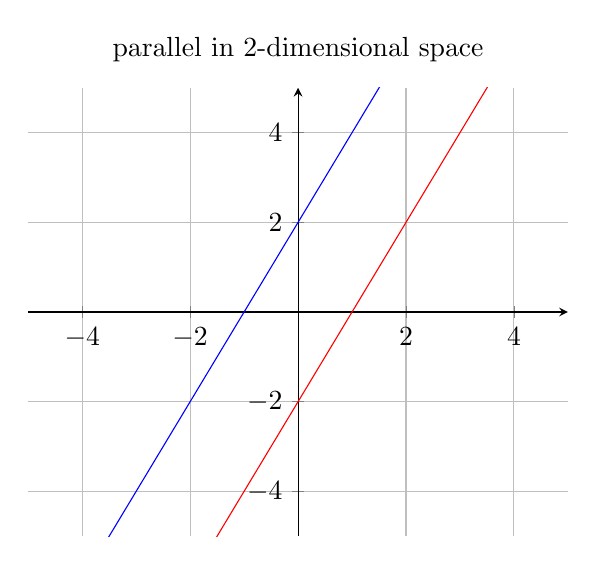
\begin{tikzpicture}
    \begin{axis}[xmin=-5, xmax=5, ymin=-5, ymax=5, axis x line=middle, axis y line=middle, title=parallel in 2-dimensional space, grid=both]
    \addplot[domain=-5:5, color=red]{2*x-2};
    \addplot[domain=-5:5, color=blue]{2*x+2};
    \end{axis}
    \end{tikzpicture}
\end{center}


\subsection{One Solution}
if each variable in the row-echelon form is a leading variable, the system has exactly one solution

\begin{center}
$\begin{vNiceArray}{cccc}[right-margin=.4em]
    \color{red}1 & 6 & $-1$ & 3 \\ 
    0 & \color{red}1 & 2 & $-2$ \\
    0 & 0 & \color{red}1 & 8 \\
    \CodeAfter 
    \UnderBrace[shorten,yshift=3pt]{3-1}{3-3}{\color{red}\text{Each variable is a leading variable}}
\end{vNiceArray}$
\end{center}
$\newline\newline$
\textbf{lines only intersect once, even they are extended infinitely}

\begin{center}
    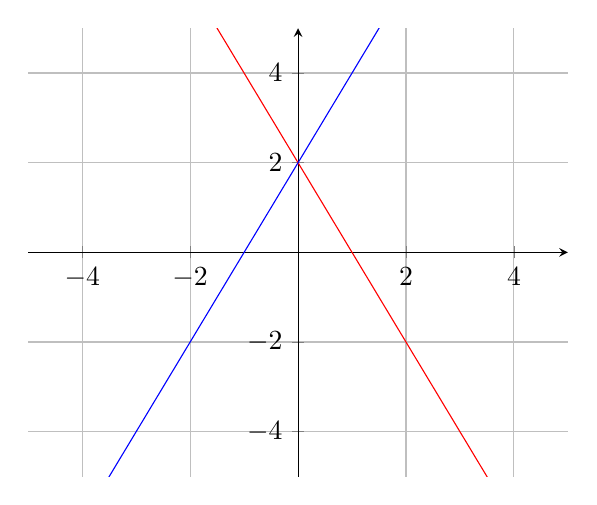
\begin{tikzpicture}
    \begin{axis}[xmin=-5, xmax=5, ymin=-5, ymax=5, axis x line=middle, axis y line=middle, grid=both]
    \addplot[domain=-5:5, color=red]{-2*x+2};
    \addplot[domain=-5:5, color=blue]{2*x+2};
    \end{axis}
    \end{tikzpicture} \\ 
\end{center}
\textbf{when extend to 3 dimensional space, situation become only intersect once with two planes} \\[5pt]
% ================================== 3 dimensional plane ===============================================
\tdplotsetmaincoords{70}{110} % I don't know why, but necessary
\begin{tikzpicture}[tdplot_main_coords,font=\sffamily]
\draw[-latex] (0,0,0) -- (4,0,0) node[left] {$x$};
\draw[-latex] (0,0,0) -- (0,4,0) node[below] {$y$};
\draw[-latex] (0,0,0) -- (0,0,4) node[left] {$z$};
\draw[fill=red,opacity=0.2] (-3,0,-3) -- (-3,0,3) -- (3,0,3) -- (3,0,-3) -- cycle;
\draw[fill=red,opacity=0.1] (-3,-3,0) -- (-3,3,0) -- (3,3,0) -- (3,-3,0) -- cycle;
\draw[thick](-3,0,0)--(3,0,0);
\node[anchor=south west,align=center] (line) at (3,3,3) {line of\\ intersection};
\draw[-latex] (line) to[out=180,in=75] (-2,0,0.05);
\end{tikzpicture}
\begin{tikzpicture}[tdplot_main_coords,font=\sffamily]
\draw[-latex] (0,0,0) -- (4,0,0) node[left] {$x$};
\draw[-latex] (0,0,0) -- (0,4,0) node[below] {$y$};
\draw[-latex] (0,0,0) -- (0,0,4) node[left] {$z$};
\tdplotsetrotatedcoords{45}{0}{0}
\begin{scope}[tdplot_rotated_coords]
\draw[fill=red,opacity=0.2] (-3,0,-3) -- (-3,0,3) -- (3,0,3) -- (3,0,-3) -- cycle;
\end{scope}
\tdplotsetrotatedcoords{90}{45}{0}
\begin{scope}[tdplot_rotated_coords]
\draw[fill=red,opacity=0.1] (-3,-3,0) -- (-3,3,0) -- (3,3,0) -- (3,-3,0) -- cycle;
\draw[thick](-3,{3/sqrt(2)},0) coordinate(x) --(3,{-3/sqrt(2)},0);
\end{scope}
\node[anchor=south east,align=center] (line) at (3,-1.5,3.5) {line of\\ intersection};
\draw[-latex] (line) to[out=0,in=135] (x);
\end{tikzpicture}
% ================================== 3 dimensional plane ===============================================

\subsection{Infinitely Many Solution = Dependent System}

\begin{center}
$\begin{vNiceArray}{cccc}[right-margin=.4em]
    1 & 2 & $-3$ & 1 \\ 
    0 & 1 & 5 & $-2$ \\
    0 & 0 & \color{red}0 & 0 \\
    \CodeAfter 
\end{vNiceArray}$ \\
\begin{center}
$\uparrow$\\
\color{red}z is not a leading variable. It is a free variable, meaning when z can take different values. According to the last row of the matrix, we are letting one dimension free,
so if vector in 3-dimension with a free variable, then it's a line in $R^3$, something like that. \\
\color{blue}
\begin{tikzpicture}[x=1cm, y=1cm, z=-0.6cm]
        % Axes
        \draw [->] (0,0,0) -- (4,0,0) node [right] {$x$};
        \draw [->] (0,0,0) -- (0,4,0) node [left] {$y$};
        \draw [->] (0,0,0) -- (0,0,4) node [left] {$z$};
        % Vectors
        \draw [->, thick] (0,0,0) -- (1,2,0);
        \draw [->, thick] (0,0,0) -- (2,4,0);
        \draw [->, thick] (0,0,0) -- (3,6,0);
        % \draw [->, thick] (0,0,0) -- (2,0,1);
        % Ticks
            \foreach \i in {1,2}
        {
        \draw (-0.1,\i,0) -- ++ (0.2,0,0);
        \draw (\i,-0.1,0) -- ++ (0,0.2,0);
        \draw (-0.1,0,\i) -- ++ (0.2,0,0);
        }
        % Dashed lines
        \draw [loosely dashed]
            (0,2,0) -- (1,2,0) -- (1,0,0)
            % (0,0,1) -- (2,0,1) -- (2,0,0)
            ;
        % Labels
         \node [right] at (1,2,0) {(1, 2, 0)};
         \node [right] at (2,4,0) {(2, 4, 0)};
         \node [right] at (3,6,0) {(3, 6, 0)};

\end{tikzpicture}
the list of vectors goes on because of the free variable... 
\end{center}
\end{center}


\section{Vector}

\textbf{Learning Feature} is the most \textbf{important} thing for any data science, then How do we learn/visualize it? \\ 
\small by vector: Apple = $[x_1, x_2, x_3, x_4, x_5]$


\subsection{Vector in $R^2$}


\begin{itemize}
    \item Geometric Description 
    \item[] 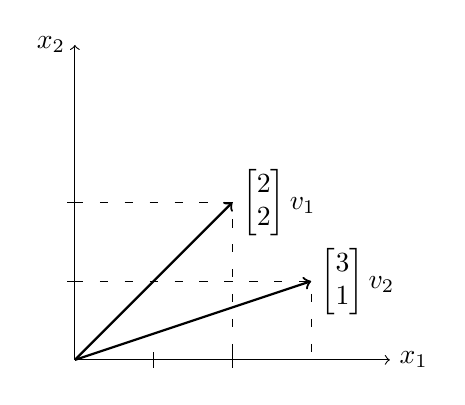
\begin{tikzpicture}[x=1cm, y=1cm]
        % Axes
        \draw [->] (0,0) -- (4,0) node [right] {$x_1$};
        \draw [->] (0,0) -- (0,4) node [left] {$x_2$};
        % Vectors itself
        \draw [->, thick] (0,0) -- (2,2);
        \draw [->, thick] (0,0) -- (3,1);
        % Ticks
            \foreach \i in {1,2}
        {
        \draw (-0.1,\i) -- ++ (0.2,0);
        \draw (\i,-0.1) -- ++ (0,0.2);
        % \draw (-0.1,\i) -- ++ (0.2,0,0);
        }
        % Dashed lines for locating the vector
        \draw [loosely dashed]
            (0,2) -- (2,2) -- (2,0)
            (0,1) -- (3,1) -- (3,0)
            ;
        % Labels, whether it's on the right or left or below or above, and many other thing
         \node [right] at (2,2) {$\begin{bmatrix}
                                    2\\2
                                   \end{bmatrix}v_1$};
         \node [right] at (3,1) {$\begin{bmatrix}
                                   3\\1
                                  \end{bmatrix}v_2$};
        \end{tikzpicture}

    \item Vector has magnitude and direction 
        \begin{itemize}
            \item[1)] magnitude: distance = $\sqrt{x_1^2 + x_2^2}$
            \item[2)] direction: $\theta=\tan^{-1}(\frac{x_2}{x_1})$

            \item[3)] representation: $\begin{cases} \vec{v_1} = 2i+2j \\ \vec{v_2} = 3i+j \end{cases}$
            \item[4)] unit vector: 
                $\begin{cases}
                    U(\vec{v_1}) = \frac{2}{\sqrt{2^2 + 2^2}}i + \frac{2}{\sqrt{2^2 + 2^2}}j \\ 
                    U(\vec{v_2}) = \frac{3}{\sqrt{3^2 + 1^2}}i + \frac{1}{\sqrt{3^2 + 1^2}}j
                \end{cases}$
        \end{itemize}
                   

\end{itemize}

\subsection{Vector in $R^n$}


\begin{itemize}
    \item Geometric Description 
    \item[] \begin{tikzpicture}[x=1cm, y=1cm, z=-0.6cm]
        % Axes
        \draw [->] (0,0,0) -- (4,0,0) node [right] {$x$};
        \draw [->] (0,0,0) -- (0,4,0) node [left] {$y$};
        \draw [->] (0,0,0) -- (0,0,4) node [left] {$z$};
        % Vectors
        \draw [->, thick] (0,0,0) -- (2,2,0);
        \draw [->, thick] (0,0,0) -- (2,0,1);
        % Ticks
            \foreach \i in {1,2}
        {
        \draw (-0.1,\i,0) -- ++ (0.2,0,0);
        \draw (\i,-0.1,0) -- ++ (0,0.2,0);
        \draw (-0.1,0,\i) -- ++ (0.2,0,0);
        }
        % Dashed lines
        \draw [loosely dashed]
            (0,2,0) -- (2,2,0) -- (2,0,0)
            (0,0,1) -- (2,0,1) -- (2,0,0)
            ;
        % Labels
         \node [right] at (2,2,0) {$\begin{bmatrix}
                                    2\\2\\0
                                   \end{bmatrix}$};
       \node [below] at (2,0,1) {$\begin{bmatrix}
                                   2\\0\\1
                                  \end{bmatrix}$};
        \end{tikzpicture}
\end{itemize}

\subsection{Linear Combinations}
\normalsize{Given vectors $v_1, v_2, \hdots, v_p$ in $R^n$ and given scalars $c_1, c_2, \hdots, c_p$, the vector \textbf{y} defined by} 
\begin{center}
    $\boldsymbol{y} = c_1\boldsymbol{v_1} + c_2\boldsymbol{v_2} + \hdots + c_p\boldsymbol{v_p}$
\end{center}
is called a \textbf{linear combination} of $\boldsymbol{v_1, v_2, \hdots, v_p}$ using weights $c_1, c_2, \hdots, c_p$

\begin{itemize}

    \item[>>] ex. Let $\boldsymbol{a_1} = \begin{bmatrix} 1 \\ 0 \\ 3 \end{bmatrix}, 
                        \boldsymbol{a_2} = \begin{bmatrix} 4 \\ 2 \\ 14 \end{bmatrix},
                        \boldsymbol{a_3} = \begin{bmatrix} 3 \\ 6 \\ 10 \end{bmatrix},
                        \boldsymbol{b} = \begin{bmatrix} -1 \\ 8 \\ -5 \end{bmatrix}$, 
                        determine if \textbf{b} is a linear combination of $\boldsymbol{a_1, a_2, \text{ and } a_3}$ 
    \item[>>] solution: check if the following equation is true
    \item[] $x_1 \begin{bmatrix} 1 \\ 0 \\ 3 \end{bmatrix} 
            + x_2 \begin{bmatrix} 4 \\ 2 \\ 14 \end{bmatrix}
            + x_3 \begin{bmatrix} 3 \\ 6 \\ 10 \end{bmatrix} =  
            \begin{bmatrix} -1 \\ 8 \\ -5 \end{bmatrix}$



\end{itemize}

\subsection{Vector Equations}

A vector equation 
\begin{center}
    $x_1 \boldsymbol{a_1}+x_2\boldsymbol{a_2}+ \hdots + x_n \boldsymbol{a_n} = b$ 
\end{center}
has the same solution set as the linear system whose augmented matrix is 
\begin{center}
    $\begin{bmatrix}
        \boldsymbol{a_1} & \boldsymbol{a_2} & \hdots & \boldsymbol{a_n} & \aug & \boldsymbol{b}
    \end{bmatrix}$
\end{center}


\subsection{Matrix Equation}

\begin{itemize}

    \item[1)] Matrix-Vector Multiplication: $\begin{bmatrix} \boldsymbol{a_1} & \boldsymbol{a_2} & \hdots & \boldsymbol{a_n} \end{bmatrix} 
        \cdot \begin{bmatrix} x_1 \\ x_2 \\ \vdots \\ x_n \end{bmatrix} = x_1\boldsymbol{a_1} + x_2\boldsymbol{a_2} + \hdots + x_n \boldsymbol{a_n}$

    \item[2)] Three Equivalent Ways of Viewing a Linear System
        \begin{itemize}
            \item[>>] as a system of linear equations
            \item[>>] as a vector equation: $x_1\boldsymbol{a_1} + x_2\boldsymbol{a_2} + \hdots + x_n \boldsymbol{a_n} = \boldsymbol{b}$
            \item[>>] as a matrix equation: $A\boldsymbol{x} = \boldsymbol{b}$
        \end{itemize}

    \item[3)] Useful Fact: The equation $A\boldsymbol{x} = \boldsymbol{b}$ has a solution if and only if \textbf{b} is a \underline{Linear Combination} of the columns of A.
\end{itemize}

\subsection{Homogeneous and Non-homogeneous Systems}

\begin{itemize}
    \item Homogeneous System 
        \begin{itemize}
            \item[>>] Definition: $A\boldsymbol{x} = \boldsymbol{0}$ \textbf{\underline{always}} has the \textbf{trivial solution} $\boldsymbol{x} = \boldsymbol{0}$;
                linear independence states only trivial solution exist, which is a different situation
            \item[>>] Nontrivial Solution: Nonzero vector solutions are called \textbf{nontrivial solutions}
        \end{itemize}

    \item Non-Homogeneous Syste 
        \begin{itemize}
            \item[>>] Definition: a Non-homogeneous system of equation is a system in which the vector of constants on the RHS of the equals sign is \textbf{non-zero}
            \item[>>] A\textbf{x}=\textbf{b}, b is a non-zero vector
            \item[>>] $\boldsymbol{b} = \begin{bmatrix} 0 \\ 3 \end{bmatrix} \neq \boldsymbol{0} $ 
        \end{itemize}

\end{itemize}
\section{Linear Independence}

A set of vectors $\{ \boldsymbol{v_1}, \boldsymbol{v_2}, \hdots, \boldsymbol{v_p} \}$ in $R^n$ is said to be \textbf{linearly independent} if vector equation
\begin{center}
    $x_1\boldsymbol{v_1} + x_2\boldsymbol{v_2} + \hdots + x_p\boldsymbol{v_p} = \boldsymbol{0}$
\end{center}
has \underline{only the trivial solution}

\begin{itemize}
    \item Is S = \{ 
        $\begin{bmatrix}
            1 \\ -4 \\ 3 
        \end{bmatrix}, 
        \begin{bmatrix}
            0 \\ 3 \\ -1
        \end{bmatrix},
        \begin{bmatrix}
            3 \\ -5 \\ 0
        \end{bmatrix}, 
        \begin{bmatrix}
            0 \\ 2 \\ -2
        \end{bmatrix}
    $ \} a linearly independent set? solve. see if A$\vec{x}=\vec{0}$ has only trivial  \\ solution:
    $\begin{bmatrix} 
        1 & 0 & 3 & 0 & \aug & 0 \\ 
        -4 & 3 & -5 & 2 & \aug & 0 \\
        3 & -1 & 0 & -2 & \aug & 0 
    \end{bmatrix}
    \sim 
    \begin{bmatrix} 
        \color{blue}1 & 0 & 3 & \color{red}0 & \aug & 0 \\ 
        0 & \color{blue}1 & 9 & \color{red}2 & \aug & 0 \\
        0 & 0 & \color{blue}-20 & \color{red}-4 & \aug & 0 
    \end{bmatrix}
    ,$ last column is the free variable column, so linearly dependent \color{red}{if we only have three entry for each vector in S, but we have more then three vector to test, 
    it's most likely LD, because once a REF is construct we gonna run out of rows than run out of columns} \color{black}
   
    \item one more example

\end{itemize}

\section{Linear Dependence}
The set $\{ \boldsymbol{v_1}, \boldsymbol{v_2}, \hdots, \boldsymbol{v_p} \}$ is said to be \textbf{linearly dependent} if there exists weights $c_1, \hdots, c_p$ are not all 0, such that
\begin{center}
    $c_1\boldsymbol{v_1} + c_2\boldsymbol{v_2} + \hdots + c_p\boldsymbol{v_p} = \boldsymbol{0}$ \\
    \color{red}! as long as weights $c_1, c_2, \hdots, c_p$ are not all zero, they could have some zero
\end{center}


\section{Vector Space}
is a non-empty set V of vector objects, give that 
\begin{itemize}
    \item[1)] zero vector($\vec{\boldsymbol{0}}$) belongs to the vector space 
    \item[2)] if there exist two vectors, $\vec{\boldsymbol{u}}$ and $\vec{\boldsymbol{v}}$ and scalar c and d then 
        \begin{itemize}
            \item[•] $\vec{\boldsymbol{u}}$ + $\vec{\boldsymbol{v}}$ is also in V
            \item[•] c$\vec{\boldsymbol{u}}$, d$\vec{\boldsymbol{v}}$ is also in V
            \item[•] c$\vec{\boldsymbol{u}}$+d$\vec{\boldsymbol{v}}$ is also in V
        \end{itemize}
\end{itemize}

\subsection{Subspace}

A subspace i.e. H is a subset of V, and if maintains the following 3 properties 

\begin{itemize}
    \item[1)] The $\vec{\boldsymbol{0}}$ must be in H. 
    \item[2)] If $\vec{\boldsymbol{u}}$, $\vec{\boldsymbol{v}}$ are two vectors in H, then $\vec{\boldsymbol{u}}$ + $\vec{\boldsymbol{v}}$ is also in H.
    \item[3)] If c is a scalar, and $\vec{\boldsymbol{v}}$ is from H, then c$\vec{\boldsymbol{v}}$ is also in H.
\end{itemize}

\subsection{Basis}
This is a Basis set for vector space (V): 
$\begin{cases} 
    \vec{\boldsymbol{v_1}} = (1,0,0)i \\
    \vec{\boldsymbol{v_2}} = (0,1,0)j \\ 
    \vec{\boldsymbol{v_3}} = (0,0,1)k \\
\end{cases}$
, and span\{ $\vec{\boldsymbol{u_1}}$, $\vec{\boldsymbol{u_2}}$, $\vec{\boldsymbol{u_3}}$ \} = $R^3$

\subsection{Span}
All linear combinations of a set of vectors: \{ $\vec{\boldsymbol{v_1}}$, $\vec{\boldsymbol{v_2}}$, $\hdots$, $\vec{\boldsymbol{v_k}}$ \} in k dimensions is called the span. 
In other words, you can build up all vectors with scalars \{ $c_1, c_2, \hdots, c_k$ \} in k dimensions with the this set of vector. \color{red} in that case 
\{$\vec{\boldsymbol{v_1}}$, $\vec{\boldsymbol{v_2}}$, $\hdots$, $\vec{\boldsymbol{v_k}}$ \} has to be \underline{linearly independent.}\color{black}

\begin{itemize}
    \item[1)] suppose we start with \{ $\vec{\boldsymbol{v_1}}$, $\vec{\boldsymbol{v_2}}$ \}, where $\vec{\boldsymbol{v_1}}$ = 
        $\begin{bmatrix}
            1 \\ 3
        \end{bmatrix}$
        and $\vec{\boldsymbol{v_2}}$ 
        $\begin{bmatrix}
            2 \\ 5
        \end{bmatrix}$
        , then span of \{ $\vec{\boldsymbol{v_1}}$, $\vec{\boldsymbol{v_2}}$ \} = $c_1 \cdot 
        \begin{bmatrix}
            1 \\ 3
        \end{bmatrix}$
        + $c_2 \cdot \begin{bmatrix} 2 \\ 5 \end{bmatrix}$, choose whatever value for $c_1, c_2$

    \item[2)] show that the vector $\begin{bmatrix} 20 \\ 4 \end{bmatrix}$ belongs to span \{ $\begin{bmatrix} 1 \\ 3 \end{bmatrix}, \begin{bmatrix} 2 \\ 5 \end{bmatrix}$ \}. 
        We solve this by augmented matrix and REF. Is the same as asking whether $\begin{bmatrix} 20 \\ 4 \end{bmatrix}$ is a linear combination of those two vectors: 
        solution is the following
        $\begin{bmatrix} 1 & 2 & \aug & 20 \\ 3 & 5 & \aug & 4 \end{bmatrix} \sim \begin{bmatrix} 1 & 0 & \aug & -92 \\ 0 & 1 & \aug & 56 \end{bmatrix}$,
        omit the intermediate step for practices purpose. we then find $c_1$ = -92 and $c_2$ = 56, verify if these two scalar could result in target vector.

    \item[3)] A = $\begin{bmatrix} 1 & 2 \\ 3 & 1 \\ 0 & 5 \end{bmatrix}$ and $ \vec{\boldsymbol{b}} 
        = \begin{bmatrix} 8 \\ 3 \\ 7 \end{bmatrix}$, Is $\vec{\boldsymbol{b}}$ in the plane spanned by A? Solve. 
        $\begin{bmatrix} 
            1 & 2 & \aug & 8 \\ 
            3 & 1 & \aug & 3 \\ 
            0 & 5 & \aug & 7 
        \end{bmatrix} \sim 
        \begin{bmatrix}
            1 & 2 & \aug & 8 \\ 
            0 & -5 & \aug & -21 \\ 
            0 & 0 & \aug & -4 
        \end{bmatrix}$, indicating the system has no solution, therefore $\vec{\boldsymbol{b}}$ is not in the plane
\end{itemize}

\subsection{Null Space}

\begin{center}
$\tikzmark{d}A\tikzmark{e}x=\tikzmark{f}B$

\begin{tikzpicture}[remember picture,overlay]
\draw[<-] 
  ([shift={(2pt,-2pt)}]pic cs:d) |- ([shift={(-10pt,-10pt)}]pic cs:d) 
  node[anchor=east] {$\scriptstyle \text{\color{red}coefficient matrix: operates on x resulting in B}$}; 
\draw[<-] 
  ([shift={(2pt,10pt)}]pic cs:e) |- ([shift={(2pt,20pt)}]pic cs:e) 
  node[anchor=south] {$\scriptstyle \text{\color{red}unknown independent variables}$}; 
\draw[<-] 
  ([shift={(2pt,-2pt)}]pic cs:f) |- ([shift={(20pt,-10pt)}]pic cs:f) 
  node[anchor=west] {$\scriptstyle \text{\color{red}dependent variables}$}; 
\end{tikzpicture}
\end{center}

\begin{itemize}
    \item Definition: The null space of an mxn matrix A is the set of all solutions to the homogeneous equation, Ax=$\vec{\boldsymbol{0}}$

    \item Metaphor: machine is A, raw material is x, B is what being made by operating A on x. Hence we set B to 0, for getting all vectors which is raw material for 
        \underline{\textbf{Null Space}}

    \item Example: A = 
        $\begin{bmatrix}  
            3 & 6 & 6 & 3 & 9 \\ 
            6 & 12 & 13 & 0 & 3
        \end{bmatrix}$,
        Find an explicit description of \textbf{Null A}. 
        \begin{itemize}
            \item[1)] solve. Ax = 0: 
                $\begin{bmatrix}  
                    3 & 6 & 6 & 3 & 9 & \aug & 0 \\ 
                    6 & 12 & 13 & 0 & 3 & \aug & 0
                \end{bmatrix} \sim \begin{bmatrix}
                    1 & 2 & 0 & 13 & 33 & \aug & 0 \\ 
                    0 & 0 & 1 & -6 & -13 & \aug & 0
                \end{bmatrix}$ \\

            \item[2)] answer. two pivots: on row 1$(x_1)$ and row 3$(x_3)$, three free variables: $x_2, x_4, x_5$, express using the free variable, because they can take any value:
                $\begin{bmatrix}
                    x_1 \\ x_2 \\ x_3 \\ x_4 \\ x_5
                \end{bmatrix} = 
                \begin{bmatrix}
                    -2x_2 - 13x_4 - 33x_5 \\ 
                    x_2 \\ 
                    0 + 6x_4 + 15x_5 \\ 
                    x_4  \\ 
                    x_5
                \end{bmatrix}$
                = $x_2\begin{bNiceMatrix}[first-row] 
                    \vec{u_1} \\
                    -2  \\ 1 \\ 0 \\ 0 \\ 0
                \end{bNiceMatrix}$ 
                + 
                $x_4\begin{bNiceMatrix}[first-row] 
                    \vec{u_2} \\
                    -13  \\ 0 \\ 6 \\ 1 \\ 0
                \end{bNiceMatrix}$ 
                + 
                $x_5\begin{bNiceMatrix}[first-row] 
                    \vec{u_3} \\
                    -33  \\ 0 \\ 15 \\ 0 \\ 1
                \end{bNiceMatrix}$

            \item[3)] also. 
                $\begin{bmatrix}
                    x_1 \\ x_2 \\ x_3 \\ x_4 \\ x_5
            \end{bmatrix} = x_2\vec{u_1} + x_4\vec{u_2} + x_5\vec{u_3} \rightarrow$ Null A = span \{$\vec{u_1}, \vec{u_2}, \vec{u_3}$\} 

        \end{itemize}
\end{itemize}

% array-like matrix labeling
% $
% \begin{blockarray}{c}
%     \color{red}u_1 \\
% \begin{block}{[c]}
%   -2  \\
%   1  \\
%   0  \\
%   0  \\
%   0  \\
% \end{block}
% \end{blockarray}
% $


\subsection{Column Space}
The column space of an mxn matrix A is the set of all possible linear combination of the columns of A  \\
\begin{itemize}
    \item Col A: A = \{ x: x is in $R^n$ and "Ax=B" \}
    \item Find a basis for Col A where A =
        $\begin{bmatrix}
            1 & 2 & 0 & 4 \\ 
            2 & 4 & -1 & 3 \\ 
            3 & 6 & 2 & 22 \\ 
            4 & 8 & 0 & 16
            \end{bmatrix}$: \\ 
            $\begin{bmatrix} A & \aug & b  \end{bmatrix}$ = 
            $\begin{bmatrix}
                1 & 2 & 0 & 4 & \aug & b_1 \\
                2 & 4 & -1 & 3 & \aug & b_2 \\ 
                3 & 6 & 2 & 22 & \aug & b_3 \\ 
                4 & 8 & 0 & 16 & \aug & b_4 
            \end{bmatrix} \sim$
            $\begin{bNiceMatrix}[last-row]
                1 & 2 & 0 & 4 & \aug & b_1^{'} \\ 
                0 & 0 & 1 & 5 & \aug & b_2^{'} \\ 
                0 & 0 & 0 & 0 & \aug & b_3^{'} \\ 
                0 & 0 & 0 & 0 & \aug & b_4^{'} \\ 
                \vec{a_1} & \vec{a_2} & \vec{a_3} & \vec{a_4} \\ 
            \end{bNiceMatrix}$, $b^{'}$ is just for simplicity, it will have scalars value and "+" or "-" sign during row reduction.

    \item Basis \{ $a_1, a_3$ \}, because they are independent variables
    \item Col A = span \{ $\vec{a_1}, \vec{a_3}$ \}
\end{itemize}

\subsection{Row Space}
The set of all linear combination of the row vectors of matrix A is called the row space: Row A \\
\indent >> ex. A = 
$\begin{bmatrix}
    -1 & 2 & 3 & 6 \\ 
    2 & -5 & -6 & -12 \\ 
    1 & -3 & -3 & -6
\end{bmatrix} \sim \begin{bmatrix}
    1 & 0 & -3 & 0 \\ 
    0 & 1 & 0 & 0 \\ 
    0 & 0 & 0 & 1
\end{bmatrix}$: Row A = span \{ $\vec{x_1}, \vec{x_2}, \vec{x_3}$ \}

\indent >> Col$A^T$ = Row A
\subsection{Linear Transformation}

A linear transformation \textbf{T} from a vector space \textbf{V} into another vector space \textbf{W} is a rule that assigns to each vector $\vec{x}$ from \textbf{V} a new unique vector $\boldsymbol{T(x)}$ 
in \textbf{W} 

\indent >> $T(\vec{v} + \vec{u}) = T(\vec{v}) + T(\vec{u})$
\\
\indent >> $T(c\vec{v}) = cT(\vec{v})$

\subsection{Kernel}

\begin{itemize}

    \item[1)] The kernel (an null space) of T is the set of all vectors $\vec{v}$ in V such that $T(\vec{v})$=0, it is a null space. The range of T is the set of all vectos in W such that $T(\vec{v})$=0. 
        Thus T(x) can be expressed as A and col(A) = Range(T)

    \item[2)] 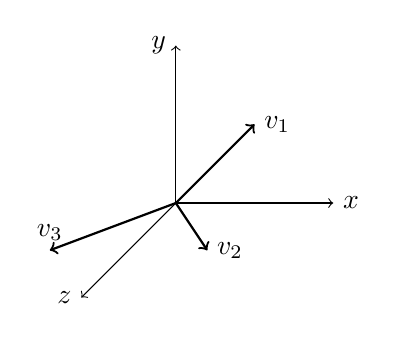
\begin{tikzpicture}[x=1cm, y=1cm, z=-0.6cm]
    % Axes
    \draw [->] (0,0,0) -- (2,0,0) node [right] {$x$};
    \draw [->] (0,0,0) -- (0,2,0) node [left] {$y$};
    \draw [->] (0,0,0) -- (0,0,2) node [left] {$z$};
    % Vectors
    \draw [->, thick] (0,0,0) -- (1,1,0);
    \draw [->, thick] (0,0,0) -- (1,0,1);
    \draw [->, thick] (0,0,0) -- (-1,0,1);
    % Ticks
        \foreach \i in {1,2};

    % Dashed lines
    % \draw [loosely dashed]
    %     (0,2,0) -- (2,2,0) -- (2,0,0)
    %     (0,0,1) -- (2,0,1) -- (2,0,0)
    %     ;

    % Labels
   \node [right] at (1,1,0) {$v_1$};
   \node [right] at (1,0,1) {$v_2$};
   \node [above] at (-1,0,1) {$v_3$};
\end{tikzpicture} \Arrow{3cm} 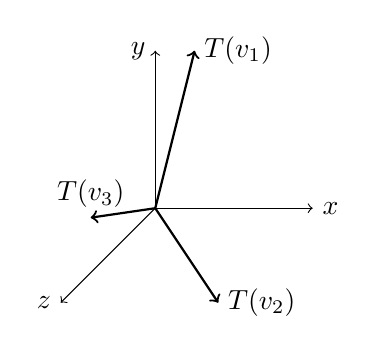
\begin{tikzpicture}[x=1cm, y=1cm, z=-0.6cm]
        % Axes
        \draw [->] (0,0,0) -- (2,0,0) node [right] {$x$};
        \draw [->] (0,0,0) -- (0,2,0) node [left] {$y$};
        \draw [->] (0,0,0) -- (0,0,2) node [left] {$z$};
        % Vectors
        \draw [->, thick] (0,0,0) -- (0.5,2,0);
        \draw [->, thick] (0,0,0) -- (2,0,2);
        \draw [->, thick] (0,0,0) -- (-0.7,0,0.2);
        % Ticks
            \foreach \i in {1,2};

        % Dashed lines
        % \draw [loosely dashed]
        %     (0,2,0) -- (2,2,0) -- (2,0,0)
        %     (0,0,1) -- (2,0,1) -- (2,0,0)
        %     ;

        % Labels
       \node [right] at (0.5,2,0) {$T(v_1)$};
       \node [right] at (2,0,2) {$T(v_2)$};
       \node [above] at (-0.7,0,0.2) {$T(v_3)$};
\end{tikzpicture}


\item[3)] From left vector space to the right vector space, we can transforming the dimension from one to another, it could be higher dimension, same or lower. The point is that 
    when we are transforming the dimension, we are trying to find new patterns from original knowledge space(left) to new knowledge space(right). 

\item[4)] \color{red}If all the vectos cluster close to zero after the transformation is perform, meaning T(x) learns nothing

\end{itemize}


\subsection{Bases for Null A and Col A}

\begin{itemize}
    
    \item To find the basis for \textbf{NULL A} $\rightarrow$ we solve $\begin{bmatrix} A & \aug& 0 \end{bmatrix}$ to find free variable: 
        $\sim 
        \begin{bmatrix}
            1 & c & 0 & \aug & b_1 \\ 
            0 & 0 & 1 & \aug & b_2 \\ 
            0 & 0 & 0 & \aug & 0 
        \end{bmatrix}, x_2$ is the free variable: $\begin{cases} x_3=b_2 \\ x_1 = b_1 - cx_2 \end{cases}$, $\vec{x} = 
            \begin{bmatrix}
                x_1 \\ x_2 \\ x_3 
            \end{bmatrix} = 
            \begin{bmatrix}
                b_1 - cx_2 \\ 
                x_2 \\ 
                b_2 + 0 \cdot x_2
            \end{bmatrix} = 
            \begin{bmatrix}
                b_1 \\ 0 \\ b_2 
            \end{bmatrix} + x_2
            \begin{bmatrix}
                -c \\ 1 \\ 0
            \end{bmatrix}$. The dimension of Nul(A) is the number of free variable of A $\rightarrow$ dim(Nul A) = $\#$ of free variable

    \item To find the basis of Col A use compute REF of the matrix A: $\begin{bmatrix} A \end{bmatrix} \sim \begin{bmatrix} 1 & 0 & 0 \\ 0 & 1 & 0 \\ 0 & 0 & 1 \end{bmatrix} \rightarrow$ dim(col A) = $\#$ pivots

\end{itemize}

\subsection{Rank Theorem}

The dimensions of the column space and row space are equal and that's called Rank
\begin{center}
    dim(Col A) = dim (Row $A^T$)
\end{center}
For an MxN matrix: \\[10pt]
\begin{center}


    $\tikzmark{a}\textbf{rank}(A)+\tikzmark{b}\textbf{dim}(\text{Nul} A)=\tikzmark{c}n$

\begin{tikzpicture}[remember picture,overlay]
\draw[<-] 
  ([shift={(2pt,-2pt)}]pic cs:a) |- ([shift={(-10pt,-10pt)}]pic cs:a) 
  node[anchor=east] {$\scriptstyle \text{\color{red} numbers of pivots}$}; 
\draw[<-] 
  ([shift={(2pt,10pt)}]pic cs:b) |- ([shift={(2pt,20pt)}]pic cs:b) 
  node[anchor=south] {$\scriptstyle \text{\color{red}numbers of free variables}$}; 
\draw[<-] 
  ([shift={(2pt,-2pt)}]pic cs:c) |- ([shift={(20pt,-10pt)}]pic cs:c) 
  node[anchor=west] {$\scriptstyle \text{\color{red}numbers of the columns}$}; 
\end{tikzpicture}
\end{center}
\indent >> Machine generates 20 dimensions, how do we know what's basic hate, and what are derived hate? -> calculating the rank and and see how many are independent vector for checking.

\subsection{Eigen Value and Eigen Vector}

A$\vec{x} = \lambda\vec{x}$, where $\lambda$ is a scalar value operator A could be reduce to constant value: $\boldsymbol{\lambda}$ is called Eigen Value, $\boldsymbol{\vec{x}}$ is called Eigen Vector

\begin{itemize}
    \item[1)] solution: A$\vec{x}$ = $\lambda\vec{x} \\
        \rightarrow A\vec{x} - \lambda\vec{x}$ = 0 \\ 
        $\rightarrow A\vec{x} - \lambda \textbf{I}\vec{x}$ = 0\\
        $\rightarrow (A-\lambda \textbf{I}) \vec{x}$ = 0 \\ 
        remember that: it's the same as saying $[A\vec{x}=\vec{B}]$: if $\vec{x}$=0 then it's trivial which is impossible because $\vec{B} \neq 0$ then $\vec{x}$ is not-trivial (Non-zero) \\
        $\rightarrow \vec{x}$ is non-trivial, then det(A-$\vec{\lambda\textbf{I}}$)=0; since ($A-\lambda\textbf{I}$) is 0, it's determinant is 0

    \item[2)] ex. Find the Eigen Value and Eigen vector for 
        $\begin{bmatrix}
            -6 & 3 \\ 
            4 & 5
        \end{bmatrix}$, solution:
        $\begin{bmatrix}
            -6 & 3 \\ 4 & 5
        \end{bmatrix} \cdot 
        \begin{bmatrix}
            x_1 \\ x_2
        \end{bmatrix} = \lambda \begin{bmatrix} x_1 \\ x_2 \end{bmatrix}$

        \begin{itemize}
            \item[•] $A-\lambda\textbf{I}\vec{x}$ = $\begin{bmatrix}
                    -6 & 3 \\ 4 & 5
            \end{bmatrix}$
            $ - \lambda \begin{bmatrix}
                1 & 0 \\ 0 & 1
            \end{bmatrix} \begin{bmatrix} x_1 \\ x_2 \end{bmatrix} = \begin{bmatrix} -6-\lambda & 3 \\ 4 & 5 - \lambda \end{bmatrix}$, 
            so as \textbf{det}
            ($\begin{bmatrix}
                -6-\lambda & 3 \\ 4 & 5-\lambda
            \end{bmatrix}$) = 0 \\

        \item[•] solve $(-6-\lambda)(5-\lambda) =0 \sim \lambda_1 = 6, \lambda_2 = -7$ \\

        \item[•] check $\lambda_1$: $\begin{bmatrix} -6 & 3 \\ 4 & 5 \end{bmatrix}
            \begin{bmatrix}
                x_1 \\ 
                x_2
            \end{bmatrix} = 
            6 \begin{bmatrix}
                x_1 \\ x_2
            \end{bmatrix} \rightarrow \begin{cases}
                -6x_1 + 3_x2 = 6x_1 \\ 
                4x_1 + 5x_2 = 6x_2 
            \end{cases} \rightarrow 
            \begin{cases}
                12x_1 = 3x_2 \\ 
                x_2 = 4x_1
            \end{cases} \rightarrow \begin{bmatrix}
            -6 & 3 \\ 4 & 5 
            \end{bmatrix} \begin{bmatrix}
            1 \\ 4
            \end{bmatrix}$ = 
            $
            \begin{bmatrix}
                -6+12 \\ 4+20
            \end{bmatrix}$ = 6
            $\begin{bmatrix}
                1 \\ 4
            \end{bmatrix}$ \\

        \item[•] check $\lambda_2$ yourself
        \end{itemize}
\end{itemize}


\section{Markov Chain}

A Markov Chain is a sequence of probability vector $x_k$, where k $\in$ N, together with stochastic matrix P, such that $x_0$ is the initial state, and $x_k = P^k x_0$ \\\\
\indent Hence, we consider that 
\begin{itemize}
    \item[] $x_1 = px_0$
    \item[] $x_2 = px_1$
    \item[] $\vdots$
    \item[] $x_n = p^{(1)}p^{(2)} \hdots p^{(k)}x_0$
    \end{itemize}




\subsection{Application of Markov Chain For ranking website}

$\rightarrow$ is the outlink(link to other website, $w_2$ doesn't have outlinks)

\begin{center}
	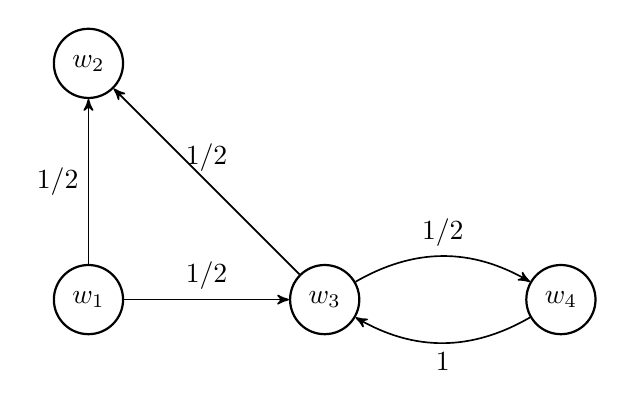
\begin{tikzpicture}[->, >=stealth', auto, semithick, node distance=3cm]
	\tikzstyle{every state}=[fill=white,draw=black,thick,text=black,scale=1]
	\node[state]    (w2)                     {$w_2$};
	\node[state]    (w1)[below of=w2]   {$w_1$};
	\node[state]    (w3)[right of=w1]   {$w_3$};
	\node[state]    (w4)[right of=w3]   {$w_4$};

    \path % path to other nodes
	(w1) edge			node{$1/2$}	(w2)
	(w1) edge			node{$1/2$}	(w3)
	(w3) edge[bend left, above]			node{$1/2$}	(w4)
	(w4) edge[bend left, below]			node{$1$}	(w3)
    (w3) edge[above]			node{$1/2$}	(w2);
	\end{tikzpicture}
\end{center}



\begin{equation*}
    \mathbf{\textbf{Perference Hypothesis}}=
  \begin{blockarray}{*{4}{c} l}
    \begin{block}{*{4}{>{$\footnotesize}c<{$}} l}
        $\tikzmark{from}w_1$ & $w_2$ & $w_3$ & $w_4$ & \\
    \end{block}
    \begin{block}{[*{4}{c}]>{$\footnotesize}l<{$}}
      0 & 0 & 0 & 0  \bigstrut[t]& $\tikzmark{to}w_1$ \\
      1/2 & 0 & 1/2 & 0  & $w_2$ \\
      1/2 & 0 & 0 & 1  & $w_3$ \\
      0 & 0 & 1/2 & 0  & $w_4$ \\
    \end{block}
  \end{blockarray}
\end{equation*}
\begin{tikzpicture}[remember picture,overlay]
    \draw[<-] 
      ([shift={(2pt,10pt)}]pic cs:from) |- ([shift={(2pt,20pt)}]pic cs:from) 
      node[anchor=south] {$\scriptstyle \text{\color{red}from}$}; 
    \draw[<-] 
      ([shift={(2pt,10pt)}]pic cs:to) |- ([shift={(2pt,20pt)}]pic cs:to) 
      node[anchor=south] {$\scriptstyle \text{\color{red}to}$}; 
\end{tikzpicture}

$\sim$ assume we the matrix for $x_n = \begin{bmatrix} 0.2 \\ 0 \\ 0.7 \\ 0.1  \end{bmatrix}$, this is the personal perference for four different websites


\subsection{Steady State}
Let P be an nxn stochastic matrix. A steady state n equilibrium vector q in $R^n$ is a vector that can be defined as follows:
\begin{center}
    $p \cdot \color{red}q\color{black} = 1 \cdot q$ \\ 
    (\color{red} a state as $x_k$ \color{black})
\end{center}
is the same as saying: Ax = $\lambda$x (where $\lambda$ = 1, q is the eigen vector and 1 is the eigen value)

\end{document}


